
\section{Prueba}


%%\subsection{Objetivo de la prueba}
%%\subsection{Herramientas utilizadas durante la prueba}
%%\subsection{Aplicación de la prueba}
%%\subsection{Conclusiones de la prueba}


%
%%\subsection{Objetivo de la prueba}
%%\subsection{Herramientas utilizadas durante la prueba}
%%\subsection{Aplicación de la prueba}
%%\subsection{Conclusiones de la prueba}

\subsection{Sprite packer}
El objetivo de esta prueba es la optimización de carga de imágenes al crear paquetes de sprites, en unity conocido como sprite packer. Se usará pruebas autómaticas con la herramienta profiles de Unity.

Una parte significativa de una textura de sprite a menudo será ocupado por el espacio vacío entre los elementos gráficos y este espacio va a resultar en memoria de video gastada en el tiempo de ejecución. Para un rendimiento optimo, lo mejor es empacar gráficas de varias texturas de sprite muy juntas dentro de una misma textura conocida como un atlas. Unity proporcionar una utilidad Sprite Packer para automatizar el proceso de generar atlases del las texturas de sprite individuales.

\begin{table}[]
	\centering
	\caption{My caption}
	\label{my-label}
	\begin{tabular}{ll}
		Pre-empaquetado & Pos-empaquetado \\
	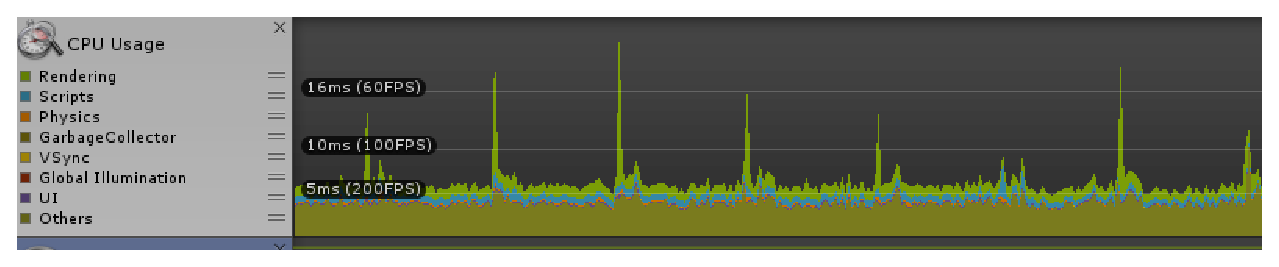
\includegraphics[width=5cm]{04ResultadosObetnidos/pruebaR/imagenes/spritespack/pre/01}	& 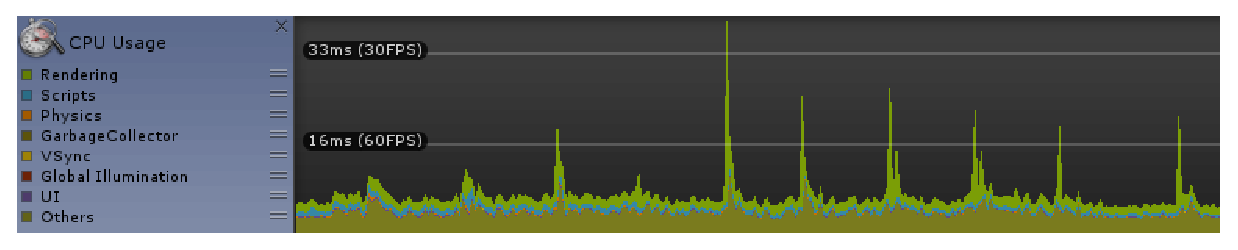
\includegraphics[width=5cm]{04ResultadosObetnidos/pruebaR/imagenes/spritespack/pos/01}                 \\
	
\includegraphics[width=5cm]{04ResultadosObetnidos/pruebaR/imagenes/spritespack/pre/02}	& 
\includegraphics[width=5cm]{04ResultadosObetnidos/pruebaR/imagenes/spritespack/pos/02}    \\
	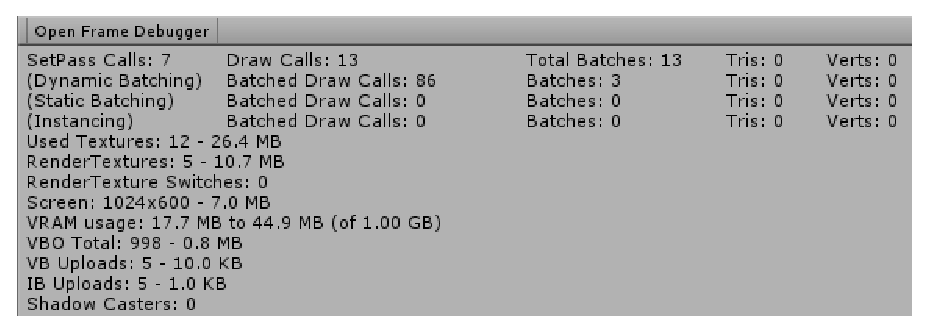
\includegraphics[width=5cm]{04ResultadosObetnidos/pruebaR/imagenes/spritespack/pre/03}	& 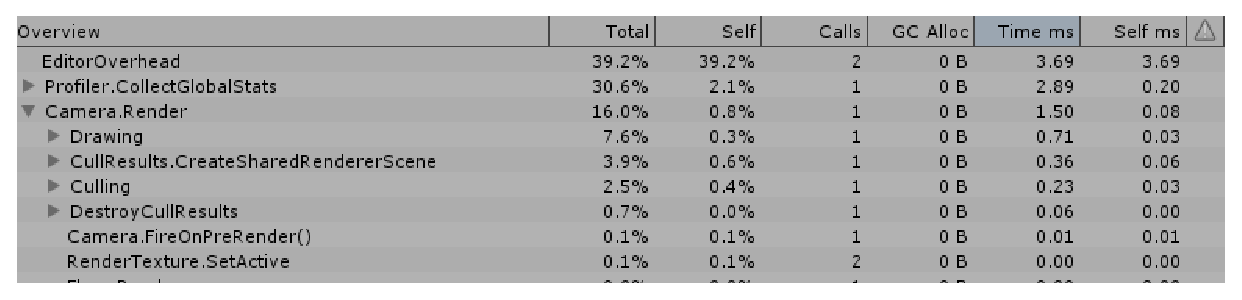
\includegraphics[width=5cm]{04ResultadosObetnidos/pruebaR/imagenes/spritespack/pos/03}       
	    
	\end{tabular}
\end{table}

Al final podemos determinar que si existe un menor porcentaje de carga en imágenes debido al empaquetado. En este caso el empaquetado fué en sprites estáticos, una mayor percepción de carga menor se puede observar al tener un empaquetado de animaciones, recordando que un movimiento en una imagen puede contener un número determinado de cuadros por segundo. Se deduce que si ha habido una optimización.

\subsection{Mecánicas del juego}
En esta parte se incluirán las pruebas de los componentes jugables que forman parte del juego. Como se desarrollan e insteractuan a lo largo del juego.
\subsubsection{Salto del jugador}
El objetivo de la prueba consiste en verificar la condición inicial del salto, en donde debe realizarse un doble salto.
Esta es una prueba funcional del juego, la herramienta a utilizar es el mismo programa de Unity, dentro del computador.
Al aplicar la prueba se detecta un salto ilimitado de veces en el jugador, debido a que el valor de verdadero o falso para permitir un salto extra no esta siendo detectado por el método de salto. Se hace un reporte final del fallo de salto extra.
\subsubsection{Plataforma en movimiento}
El objetivo de la prueba es comprobar que funcione la plataforma con movimiento tanto horizontal como vertical como se ha determinado. La herramienta a utilizar sigue siendo dentro del computador Unity.
Como prueba dentro del funcionamiento del juego el jugador se posiciona sobre la plataforma, la plataforma se desplaza de forma adecuada y en la dirección establecida, tanto el movimiento horizontal como el movimiento vertical. Pero se detecta que el desplazamiento es independiente al personaje, por lo que el jugador debe manualmente seguir la trayectoria de la plataforma, en este caso particular, la plataforma horizontal. Mientras que en el caso de la plataforma vertical se detecta una disminución de velocidad al realizar una ascención y un aumento de velocidad al descender. Se concluye que los componentes funcionan de manera independiente en cuanto a su movimiento, la solución a proponer consistiría en un código por parte de la plataforma en movimiento que cuando detecte al jugador le aplique la misma velocidad que este realice sumándosela a la que pudiera el jugador tener en ese momento y esto sería solo al contacto de la plataforma.

\subsection{Dinámicas del juego}
En esta parte las pruebas van dirigidas a las situaciones que crea el jugador con lo que se le hes permitido dentro del videojuego.
\subsubsection{Salto bajo}
El objetivo de la prueba consiste en entender la percepción del usuario ante las acciones que realiza el personaje dentro del juego. La herramienta a utilizar es en el computador en el programa Unity. El jugador se presenta en diferentes escenarios de los niveles para que pueda moverse a voluntado propia dentro de lo que establece el juego. Las situaciones a las que se presenta el jugador abarcan saltar en plataformas estáticas, plataformas móviles, camino horizontal y camino ascendente. Al final el usuario reporta que en su propia percepción el salto o elevación del personaje es menor al que le gustaría o en algunas ocasiones al que necesita. Las soluciones a proponer consisten en aumentar la variable que controla el movimiento ascendente del jugador o la variable que controla la gravedad proporcionada en el juego.  
\subsubsection{Instrucciones del juego}
El objetivo de la prueba consiste en entender la percepción del usuario ante las acciones que realiza dentro del nivel introductorio del juego. La herramienta a utilizar es en el computador en el programa Unity. Al usuario se le presenta el nivel introductorio del juego para que termine con este mismo. Al final reporta que por prueba y error ha sabido el funcionamiento de los botones que se le presenta, según a opinión del usuario le gustaría dentro del juego una demostración o explicación de los mismos botones y lo que hacen. Al final se propone como solución dentro de los mismos diálogos explicar el funcionamiento de los botones, o el realizar un video explicativo de los botones o indicarle al usuario que realice actividades determinadas para la prueba de los botones. 
\subsubsection{Desbloqueo de personas}
El objetivo de la prueba consiste en entender la percepción del usuario ante las acciones que realiza dentro del nivel introductorio del juego. La herramienta a utilizar es en el computador en el programa Unity. Al usuario se le presenta como situación seguir avanzando al siguiente nivel dentro del nivel introductorio, donde en una parte el jugador debe desbloquear al menos cinco diálogos. El jugador reporta que aunque sea el mismo diálogo que active una y otra vez, este se contabiliza sin ningun problema. La solución a proponer es colocar una variable de verdadero y falso para indicar si el diálogo ha sido activado y así no contabilizarlo nuevamente.


\subsection{Estética del juego}
En esta parte las pruebas van dirigidas a la respuesta del jugador ante lo que se le presenta directamente como interacción dentro del juego, ya sea auditiva o visualmente.
\subsubsection{Ilustraciones de items}
El objetivo de la prueba consiste en entender la percepción del usuario ante lo que se le muestra a lo largo del juego. La herramienta a utilizar es en el computador en el programa Unity. Dentro de los niveles impares el jugador reporta un poco confuso a primera vista el item que incrementa el tonalli, al no reconocer que objeto lo representaba. El objeto a querer mostrar es una flor de vainilla, al mostrar la imagen por separado al jugador y presentarlo en un tamaño más grande el usuario reporta como comfuso las ramas u hojas de la imagen a lado de la flor. Como propuesta de solución se tiene la eliminación de las ramas u hojas de la imagen, dejando solo la flor visible o hacer mucho más grande la imagen presente en el juego.
\subsubsection{Menú principal}
El objetivo de la prueba consiste en entender la percepción del usuario ante lo que se le muestra en el menú principal. La herramienta a utilizar es en el computador en el programa Unity.
=======
%\begin{table}[prueba01]
%	\centering
%	\caption{My caption}
%	\label{my-label}
%	\begin{tabular}{ll}
%		\multicolumn{2}{l}{Prueba 01} \\
%		Objetivo                  &  asdasdasd \\
%		Herramientas utilizadas   &  asdasdasd \\
%		Aplicación                &  asdasdasd \\
%		Conclusiones              &  adasdasd
%	\end{tabular}
%\end{table}

